
\documentclass[slides]{beamer}
\usepackage[]{graphicx, color}

%\usepackage{pgfpages}
%\pgfpagesuselayout{2 on 1}[border shrink=5mm]
%\pgfpageslogicalpageoptions{1}{border code=\pgfusepath{stroke}}
%\pgfpageslogicalpageoptions{2}{border code=\pgfusepath{stroke}}


\mode<presentation>
{
	%\usetheme[secheader]{Boadilla}
	%\usecolortheme[rgb={.835, .102,.169}]{structure}  
	\usetheme[width=0cm]{Goettingen}
	%\setbeamercovered{transparent}
}
\setbeamertemplate{navigation symbols}{}
\setbeamertemplate{footline}[frame number]

\definecolor{blue2}{rgb}{0.278,0.278,0.729} 
\newcommand{\blue}[1]{\textcolor{blue2}{#1}}
\newcommand{\white}[1]{\textcolor{white}{#1}}
\newcommand{\red}[1]{\textcolor{red}{#1}}
\newcommand{\xbar}{\overline{x}}
\newcommand{\ybar}{\overline{y}}
\newcommand{\phat}{\widehat{p}}


\usepackage{hyperref}

\title{Lecture 11.1: Linear Regression Part II}
\author{Chapter 7.2-7.4}
\date{2014/04/14}


\begin{document}
%------------------------------------------------------------------------------
\begin{frame}
\titlepage
\end{frame}
%------------------------------------------------------------------------------


%%------------------------------------------------------------------------------
%\begin{frame}[fragile]
%\frametitle{Announcement}
%
%Who here likes ``debugging'' R code?
%\begin{itemize}
%\pause\item Marissa Mayer: \blue{\url{http://www.crunchbase.com/person/marissa-mayer}}
%\pause\item Eric Roberts: \blue{\url{http://www.newsweek.com/googles-marissa-mayer-girls-can-be-geeks-too-68965}}
%\pause\item Tomorrow's math colloquium: \blue{\url{http://academic.reed.edu/math/seminars/index.html}}
%\end{itemize}
%
%\end{frame}
%%------------------------------------------------------------------------------


%%------------------------------------------------------------------------------
%\begin{frame}[fragile]
%\frametitle{Quiz 9}
%
%\blue{\url{http://www.nature.com/news/scientific-method-statistical-errors-1.14700}}
%
%\begin{itemize}
%\pause\item \blue{Question 1}: What is p-hacking?\\
%\pause \blue{Answer 1}: Data-dredging AKA ``trying multiple things until you get the desired result'' \blue{\url{http://simplystatistics.org/2013/08/26/statistics-meme-sad-p-value-bear/}}
%%-------------
%\pause\item \blue{Question 2}: Say a scientist obtains a p-value of 0.01.  An incorrect interpretation of this is that it is the probability of a ``false alarm'' (type I error)...  If one wants to make a statement about this being a false alarm, what additional piece of information is required?\\
%\pause \blue{Answer 2}: The plausibility of the hypothesis being tested for.  
%\end{itemize}
%
%\end{frame}
%%------------------------------------------------------------------------------


%%------------------------------------------------------------------------------
%\begin{frame}[fragile]
%\frametitle{Quiz 10}
%
%\blue{\url{http://opinionator.blogs.nytimes.com/2013/04/25/what-do-scientific-studies-show/?_php=true&_type=blogs&_r=0}}
%
%\begin{itemize}
%\pause\item \blue{Question 1}: According to the article, why do scientists even bother with correlational/observational studies, when no notions of causality can be established?\\
%\pause \blue{Answer 1}: They are excellent starting points for deciding which hypotheses to evaluate with the more rigorous randomized controlled experiment.  
%%-------------
%\pause\item \blue{Question 2}: The article argues that various scientific disciplines should set professional labeling standards for material discussed in popular media.\\
%\pause \blue{Answer 2}:
%\begin{enumerate}
%\item preliminary result
%\item large-scale observational study
%\item large-sample randomized controlled test
%\item well-established scientific law that we know how to apply in a wide range of conditions
%\end{enumerate}
%\end{itemize}
%
%\end{frame}
%%------------------------------------------------------------------------------


%------------------------------------------------------------------------------
\begin{frame}[fragile]
\frametitle{Questions for Today: Example From Text}
\begin{itemize}
\pause\item Data: random sample of 50 students in the 2011 freshman class of Elmhurst College in Illinois.
\pause\item Explanatory variable: Family income
\pause\item Outcome variable: Gift Aid (financial aid that is a gift, not a loan)
\end{itemize}

\begin{center}
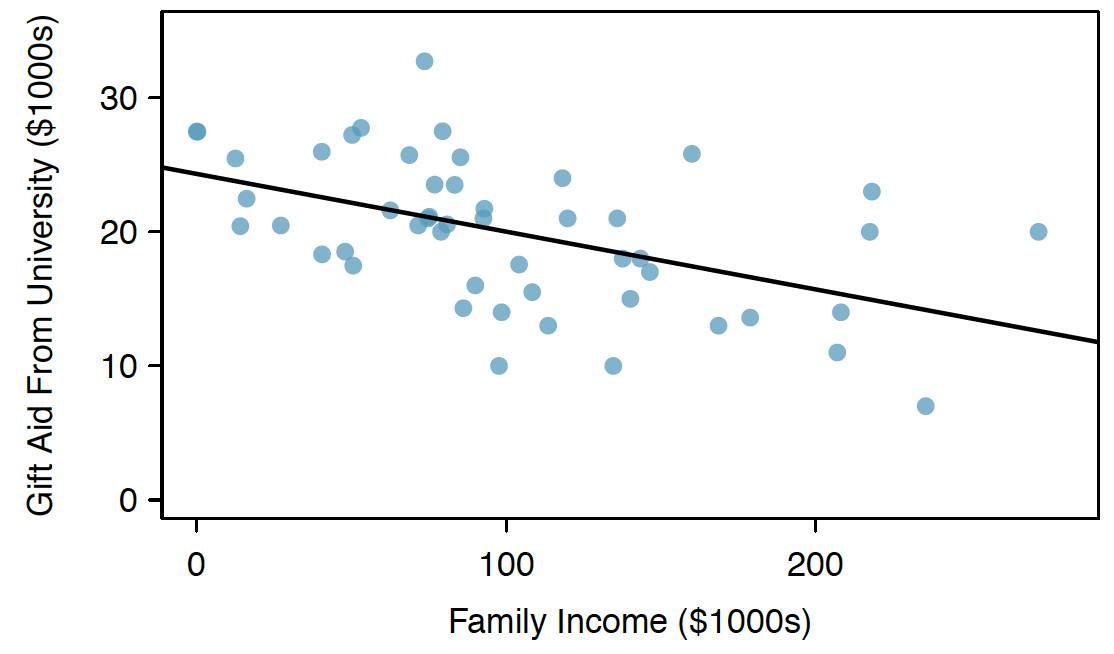
\includegraphics[width=0.8\textwidth]{regression.png}
\end{center}

\end{frame}
%------------------------------------------------------------------------------


%------------------------------------------------------------------------------
\begin{frame}[fragile]
\frametitle{Questions for Today: Example From Text}
Using these values,
\begin{center}
\begin{tabular}{l|rr}
& family income & gift aid \\
& in \$1000's (x) & in \$1000's (y) \\ 
\hline
mean & $\overline{x}=101.8$ & $\overline{y}=19.94$ \\ 
sd & $s_x=63.2$ & $s_y=5.46$ \\ 
\hline
 &  & $R=-0.499$ \\ 
\hline
\end{tabular}
\end{center}
they fit the \blue{least-squares line}:
\pause
\begin{eqnarray*}
\widehat{y} &=& b_0 + b_1 x\\
\mbox{i.e. }\widehat{\mbox{aid}} &=& 24.3 - 0.0431 \times \mbox{family\_income}
\end{eqnarray*}
What do $24.3$ and $-0.0431$ mean?

\end{frame}
%------------------------------------------------------------------------------


%------------------------------------------------------------------------------
\begin{frame}[fragile]
\frametitle{Point Estimates of Intercept}
\blue{Point estimate of intercept $b_0$}: 24.3 (in \$1000's) describes the average aid if the family had no income.  

\vspace{0.25cm}
\pause
In this case it is relevant since some families make no income, but the intercept may have little or no practical value if there are no observations near $x=0$.  

\end{frame}
%------------------------------------------------------------------------------


%------------------------------------------------------------------------------
\begin{frame}[fragile]
\frametitle{Point Estimates of Slope}
\blue{Point estimate of slope $b_1$}: More interesting. It describes the \blue{relationship} between $x$ and $y$

\vspace{0.5cm}
\pause
For this example, for each additional \$1000 of family income, we would \blue{expect} a student to receive a net difference of $\$1000 \times (-0.0431) = -\$43.10$ in aid on average.   

\vspace{0.5cm}
\pause
Again, even though we've labeled aid as the outcome variable, we are not positing a causal relationship, just an association.  


\end{frame}
%------------------------------------------------------------------------------


%------------------------------------------------------------------------------
\begin{frame}[fragile]
\frametitle{Extrapolate with Care}
Definition of \blue{extrapolation}:  extend the application of a method or conclusion to an unknown situation by assuming that existing trends will continue or similar methods will be applicable.

\vspace{0.5cm}
\pause
What would be the gift aid given to a family with one million dollars ($x=1000$) in family income?
\[
24.3 - 0.0431 \times 1000 = -18.8
\]
The school will take \$18,800 dollars away from you?  


\end{frame}
%------------------------------------------------------------------------------


%------------------------------------------------------------------------------
\begin{frame}[fragile]
\frametitle{Categorical Predictor $x$ With Two Levels}
$x$ need not just be a numerical value; it can also be categorical.  

\vspace{0.25cm}
\pause
Ex: Ebay price for the video game Mario Kart. We convert the categorical $x$ into a \blue{indicator variable} $\mbox{cond\_new}$ which has 2 \blue{levels}:
\begin{enumerate}
\item $x=0$:  game is used. This is the \blue{baseline} level.
\item $x=1$:  game is new.
\end{enumerate}
\pause
The linear model is thus
\[
\widehat{\mbox{price}} = b_0 + b_1 \times \mbox{cond\_new}
\]

\end{frame}
%------------------------------------------------------------------------------


%------------------------------------------------------------------------------
\begin{frame}[fragile]
\frametitle{Categorical Predictor $x$ With Two Levels}

\begin{center}
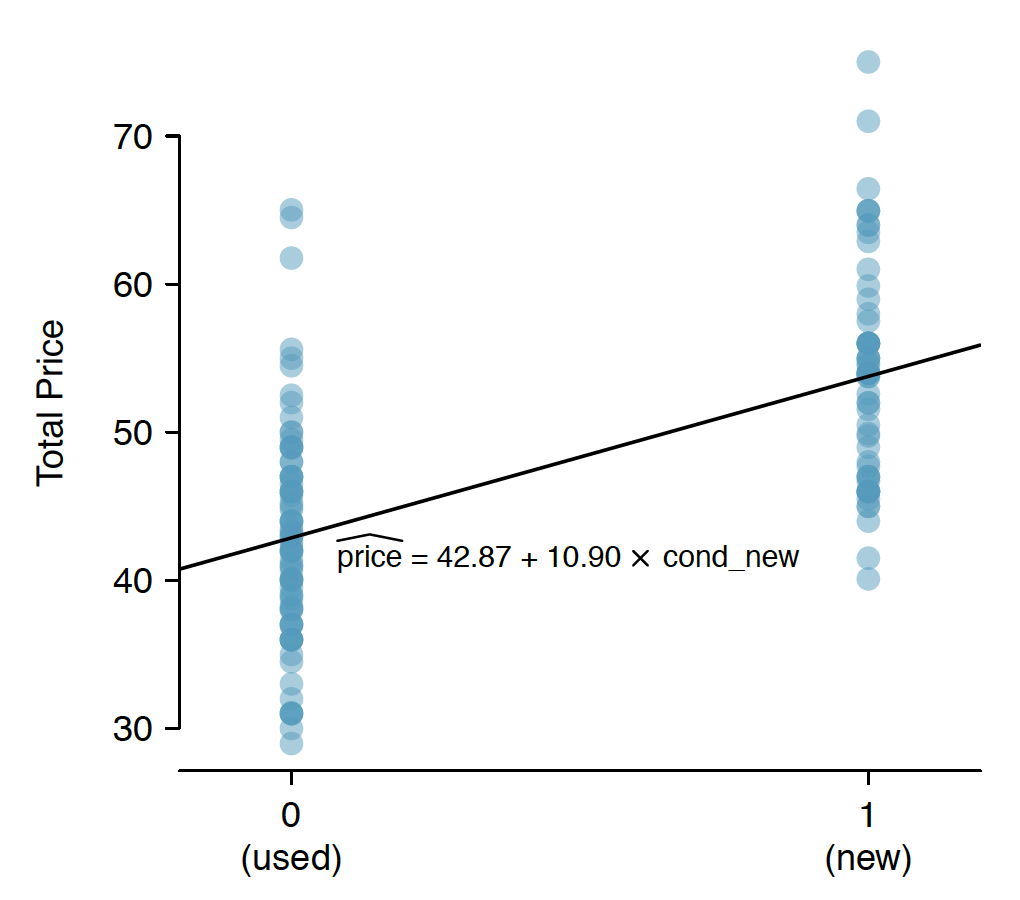
\includegraphics[width=0.8\textwidth]{mario_kart.png}
\end{center}

\end{frame}
%------------------------------------------------------------------------------


%------------------------------------------------------------------------------
\begin{frame}[fragile]
\frametitle{Categorical Predictor $x$ With Two Levels}
The least-squares line is
\[
\widehat{\mbox{price}} = 42.87 + 10.90 \times \mbox{cond\_new}
\]
\pause
So when the game is
\begin{itemize}
\item Old, we have $x=0$, so the fitted value is $\$42.87 + \$0 = \$42.87$
\item New, we have $x=1$, so the fitted value is $\$42.87 + \$10.90 = \$53.77$
\end{itemize}
\pause
This can be generalized for predictor variables $x$ with more than two levels, but this requires a different encoding of $x$.

\end{frame}
%------------------------------------------------------------------------------


%------------------------------------------------------------------------------
\begin{frame}[fragile]
\frametitle{Types of Outliers in Linear Regression}
\begin{center}
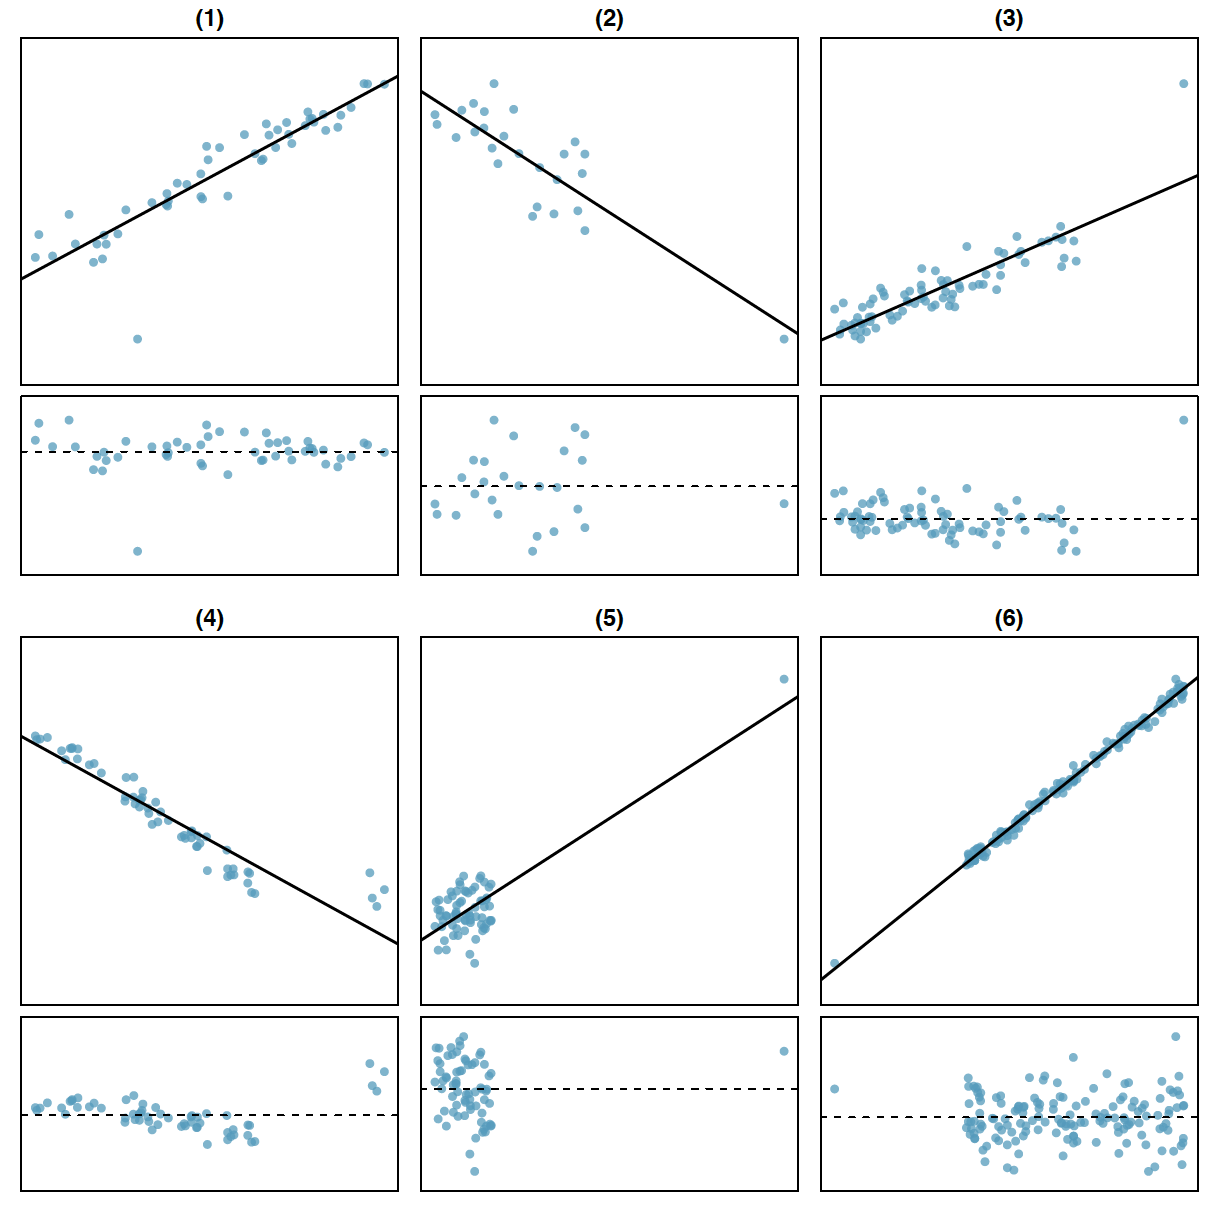
\includegraphics[height=0.8\textheight]{outliers.png}
\end{center}
\end{frame}
%------------------------------------------------------------------------------


%------------------------------------------------------------------------------
\begin{frame}[fragile]
\frametitle{Types of Outliers in Linear Regression}
Especially in cases 3 and 5, the outliers seem to be pulling the least-squares line towards them.

\vspace{0.5cm}
\pause
Points that fall horizontally away from the center of the cloud tend to pull harder on the line, so we call them points with high \blue{leverage}, i.e. large influence.  

\end{frame}
%------------------------------------------------------------------------------


%------------------------------------------------------------------------------
\begin{frame}[fragile]
\frametitle{Next Example}

Are Higher Movie Budgets Associated with Higher IMDB Ratings for Movies Made from 1980-2005?  Guesses?

\vspace{0.5cm}

\pause But first, are the changes from
\begin{itemize}
\item 100 to 200
\item 100,100 to 100,200
\end{itemize}
the same?


\end{frame}
%------------------------------------------------------------------------------


%------------------------------------------------------------------------------
\begin{frame}[fragile]
\frametitle{Next Example}
We consider a $\log_{10}$ transformation:

\begin{center}
  \begin{tabular}{cc|c|cc}
    $x$ & $y$ & $y-x$ & $\frac{y}{x}$ & $\log_{10}\left(\frac{y}{x}\right)$\\ 
\hline
    100 & 200 & 100 & 2 & 0.301\\ 
    100100 & 100200 & 100 & 1.000999 & $0.00004342$\\ 
    \pause 100000 & 200000 & 100000 & 2& \blue{0.301} \\ 
  \end{tabular}
\end{center}

\pause Recall that $\log_{10}\left(\frac{y}{x}\right) = \log_{10}(y) - \log_{10}(x)$

\vspace{0.5cm}

\pause So we are considering \blue{multiplicative} changes, and not \blue{additive} changes.


\end{frame}
%------------------------------------------------------------------------------


%%------------------------------------------------------------------------------
%\begin{frame}[fragile]
%\frametitle{Midterm I Scores}
%Recall the analysis where we asked:  Did students who finished early do better?
%\begin{itemize}
%\item Explanatory variable $x$: submission rank
%\item Response variable $y$: midterm score
%\end{itemize}
%
%\begin{center}
%\includegraphics[width=0.7\textwidth]{midtermI.png}
%\end{center}
%
%\end{frame}
%%------------------------------------------------------------------------------
%
%
%%------------------------------------------------------------------------------
%\begin{frame}[fragile]
%\frametitle{Midterm I Scores}
%The output of the regression analysis:  
%\begin{table}[ht]
%\centering
%\begin{tabular}{r|rrrr}
%  \hline
% & Estimate & Std. Error & t value & Pr($>$$|$t$|$) \\ 
%  \hline
%(Intercept) & 20.5871 & 0.9460 & 21.76 & 0.0000 \\ 
%  submit rank & -0.0317 & 0.0516 & -0.61 & 0.5444 \\ 
%   \hline
%\end{tabular}
%\end{table}
%
%\vspace{0.25cm}
%\pause
%The point estimate $b_0 = 20.58$ of the intercept coefficient by itself doesn't mean anything: fitted score for someone who submitted at rank 0?
%
%\end{frame}
%%------------------------------------------------------------------------------
%
%
%%------------------------------------------------------------------------------
%\begin{frame}[fragile]
%\frametitle{Interpretation of Midterm I Scores Analysis Results}
%
%The point estimate $b_1=-0.0317$ of the slope coefficient means: for every increase in one in submission rank, we observe on average a \blue{decrease} of 0.0317 in the midterm I score.  
%
%\vspace{0.25cm}
%\pause
%Since $b_1$ is a point estimate based on $n=31$ $(x_i, y_i)$ pairs, we can associate a standard error (0.0516).  
%
%\vspace{0.25cm}
%\pause
%We conduct a two-sided hypothesis test of:
%\begin{eqnarray*}
%&& H_0: \beta_1 = 0\\
%\mbox{vs}&& H_A: \beta_1 \neq 0 
%\end{eqnarray*}
%thus the t-value is
%\[
%T = \frac{\mbox{point estimate}-\mbox{null value}}{\mbox{standard error}} = 
%\frac{-0.0317-0}{0.0516} = -0.61
%\]
%
%\vspace{0.25cm}
%\pause
%Pr($>$$|$t$|$) indicates the two-sided p-value of 0.5444. 
%
%\end{frame}
%%------------------------------------------------------------------------------
%
%
%%------------------------------------------------------------------------------
%\begin{frame}[fragile]
%\frametitle{Residuals Plot}
%\begin{center}
%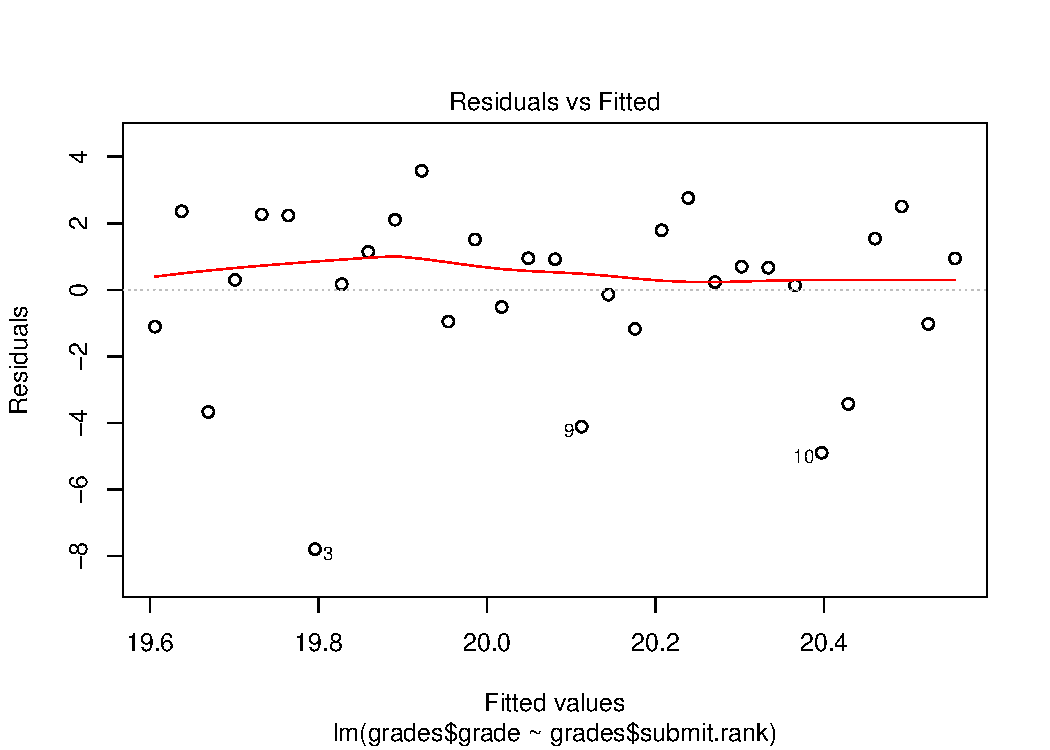
\includegraphics[width=\textwidth]{resid1.pdf}
%\end{center}
%\end{frame}
%%------------------------------------------------------------------------------
%
%
%%------------------------------------------------------------------------------
%\begin{frame}[fragile]
%\frametitle{QQ-Plot of (Standardized) Residuals}
%\begin{center}
%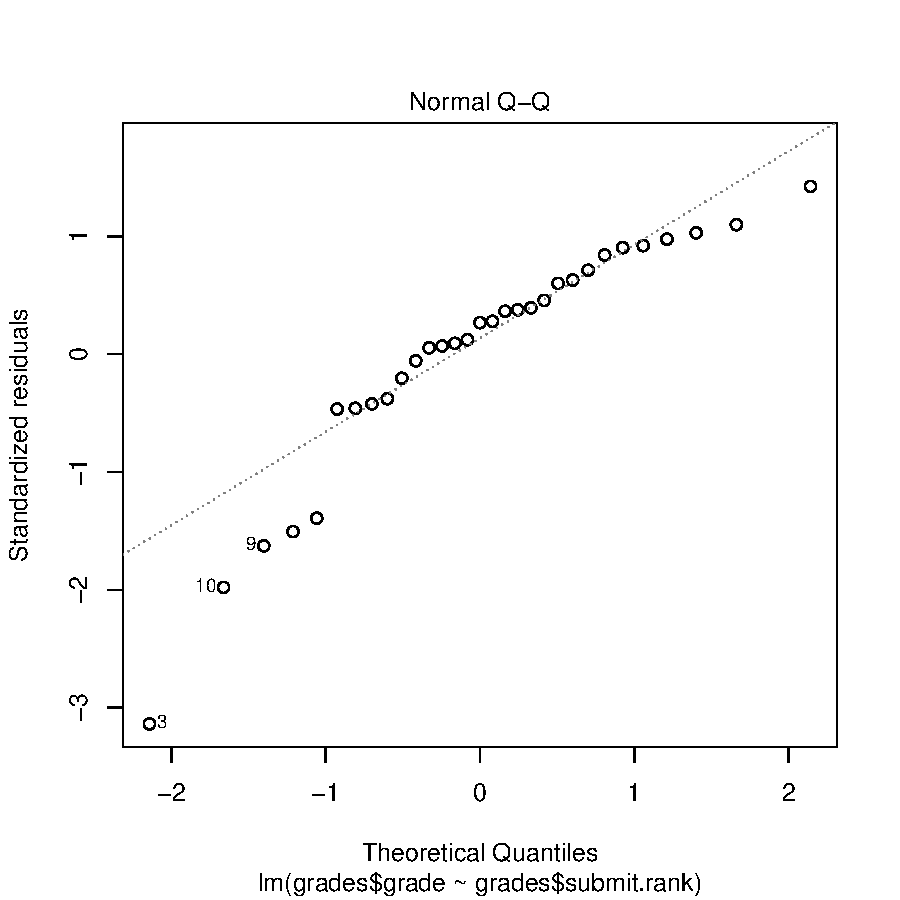
\includegraphics[width=0.7\textwidth]{resid2.pdf}
%\end{center}
%\end{frame}
%%------------------------------------------------------------------------------


%------------------------------------------------------------------------------
\begin{frame}[fragile]
\frametitle{Next Time}

Multiple Regression:  As opposed to \blue{simple linear regression} where there is only one predictor/explanatory variable $x$, we now consider \blue{many} variables $x_1, x_2, \ldots$

\end{frame}
%------------------------------------------------------------------------------


\end{document}












